\documentclass[twocolumn]{article}


\usepackage{fullpage}
\usepackage{amsmath}
\usepackage{graphicx}
\usepackage{float}
\usepackage{natbib}
\usepackage[capitalise,noabbrev]{cleveref}
\usepackage{enumitem}
\usepackage{multirow}

\newcommand{\img}[1]{\includegraphics[width=3in]{#1}}
\newcommand{\ep}{\varepsilon}

\begin{document}
	
\twocolumn[{
	\centering
	\LARGE General Bayesian Marginal Likelihood Estimation Using Iterative Density Estimation\\[1.5em]
	\large Taylor McKenzie\\[1.5em]
}]

\begin{abstract}
	Bayesian statistics provides a very general, well-founded, and intuitive framework for model selection. Any exclusive models that permit a proper posterior distribution can be compared via Bayes' factors, and the probability that any given model from a set of potential models is correct can be calculated. However, it can be difficult to estimate Bayes' factors due to difficulties in computing a model's marginal likelihood. Methods have been developed to make this problem computationally feasible for models that fit with Gibbs or Metropolis-Hastings samplers \citep{ChibJeliazkov}. Unfortunately, many models cannot be fit using Gibbs sampling, and Metropolis-Hastings sampling may be much slower than newer algorithms such as No U-Turn Sampling \citep{NUTS}. This research develops a general algorithm to estimate marginal likelihood and, by extension, Bayes' factors using iterative kernel density estimation. Using this algorithm with No U-Turn Sampling can produce unbiased, lower variance estimates of marginal likelihood for a broader class of models than those from other methods for similar numbers of sampling iterations.
\end{abstract}

\section{Introduction}

\section{Literature Review}

\subsection{Model Selection}
%Citations here: 
%Classical: Greene, Akaike, Schwarz (SBIC)
%Cross-validation: Allen, Golub, Kohavi (machine learning), Arlot (survey of methods)
%Bayeisan: Chib, Chib & Jeliazkov, Kass & Raftery (Bayes' factor), George (mixed model selection), Berger (?)

Density estimation could theoretically be used to estimate marginal likelihood. However, this method has not been feasible historically due to practical issues with many kernel density estimators, described in greater detail in the following subsection.

\subsection{Kernel Density Estimation}
%Citations here:
%Silverman (most density estimation, including standard, adaptive, etc.)
%Portnoy (application of adaptive KDE and some references)
%Beran (adaptive rank estimator)

%Idea for this section: Lay out KDE basics (formula), illustrate weakness (bias in density estimates), state how adaptive KDE fixes.

\subsection{Markov Chain Monte Carlo Samplers}
%Citations here:
%Gelfand & Smith (overview)
%Chib & Greenberg (M-H), Geman (Gibbs), Tanner & Wong (data augmentation), Rubin (importance sampling)

\section{Theory and Method}

As mentioned previously, models estimated in the Bayesian framework can be compared via their marginal likelihoods. For two models $M_j$ and $M_k$, the relative goodness-of-fit of $M_k$ over $M_j$, called the Bayes' factor, is the ratio of the marginal likelihoods of each model, expressed as
\begin{equation}
	\frac{m(y|M_k)}{m(y|M_j)}.
\end{equation}
The marginal likelihood of $M_k$ can be written as
\begin{equation}
	m(y|M_k) = \frac{f(y|\theta, M_k)p(\theta|M_k)}{p(\theta|y, M_k)},
\end{equation}
where $\theta$ are parameters of the model, $f(y|\theta, M_j)$ is the likelihood of the data, $p(\theta|M_j)$ is the value of the prior density, and $p(\theta|y, M_j)$ is the posterior density. As noted by \cite{Chib}, this identity holds for each $\theta$, and while the values of the likelihood and prior density are typically known (because they are specified to estimate the model), the value of the posterior density is usually unknown, motivating the development of many Markov Chain Monte Carlo (MCMC) techniques to sample from the posterior distribution. In practice, the marginal likelihood must be estimated at a point $\theta^*$ via estimation of the posterior density. As noted by \cite{Chib}, using $\theta^*$ from a high-density region of the posterior can reduce the variance of marginal likelihood estimates.

While a number of methods have been developed to estimate the value of the posterior density in certain cases, a simple and general approach is to use kernel density estimation (KDE), which can be used to construct and estimate values of a density function from samples of a random variable. Since all MCMC methods produce samples of $\theta|y, M_k$, this method can be used for any MCMC algorithm. Howevef, there are two fundamental issues that complicate this approach. First, many standard KDE procedures produce biased estimates of the density function, systematically underestimating values in high-density regions and overestimating values in low-density regions \citep{SilvermanDE}. Fortunately, this is easily remedied via use of more sophisticated KDE methods, such as adaptive KDE.

The other issue complicating the use of KDE to estimate posterior densities is based in the curse of dimensionality. In practice, the posterior density is often a function of several parameters, and KDE becomes less reliable as the number of dimensions and is often completely infeasible for more than five dimensions. To illustrate a solution, first denote the parameter vector as $\theta = (\theta_1, \theta_2, ..., \theta_P)',$ where $P$ is the total number of parameters. Using laws of conditional probability (and now omitting the conditional on model $M_k$), we can write the marginal likelihood as
\begin{align}
	p(\theta|y)
	&= p(\theta_1, ..., \theta_P|y) \\
	&= p(\theta_1|\theta_2, ..., \theta_P, y)\times p(\theta_2, ..., \theta_P|y) \\
	&= p(\theta_1|\theta_2, ..., \theta_P, y)\times p(\theta_2|\theta_3, ..., \theta_P, y) \\ &\qquad\times p(\theta_3, ..., \theta_P|y) \\
	&= ... \\
	&= p(\theta_1|\theta_2, ..., \theta_P, y)\times p(\theta_2|\theta_3, ..., \theta_P, y)\\ &\qquad\times ...\times p(\theta_P|y).
\end{align}
So, the value of the posterior density can be estimated using the following procedure:
\begin{enumerate}[noitemsep]
	\item Draw samples of $\theta|y$ using an MCMC algorithm.
	\item Choose $\theta^*$ from a high-density region of $\theta|y$, such as the sample mean or maximum a posteriori.
	\item Estimate the log-density of $\theta_P|y$ at $\theta_P^*$ using adaptive KDE, denoting that value $\ln \hat{p}(\theta_P^*|y)$.
	\item For each $i$ from $P-1, ..., 1$:
		\begin{enumerate}
			\item Re-estimate the model, setting $(\theta_{i+1}, ..., \theta_P) = (\theta_{i+1}^*, ..., \theta_P^*)$, to obtain draws of $(\theta_1, ..., \theta_i)|(\theta_{i+1}^*, ..., \theta_P^*), y$.
			\item Estimate the log-density of $\theta_i|\theta_{i+1}^*, ..., \theta_P^*, y$ at $\theta_i^*$ using adaptive KDE, denoting that value $\ln \hat{p}(\theta_i^*|\theta_{i+1}^*, ..., \theta_P^*, y)$.
		\end{enumerate}
	\item Find the sum of each of the estimated partial log-densities to arrive at an estimate for the overall log-posterior density, denoted $\ln \hat{p}(\theta^*|y)$.
\end{enumerate}

This iterative formulation is by no means novel (a similar formulation was used in \cite{Chib} and \cite{ChibJeliazkov} for Gibbs and Metropolis-Hastings (M-H) samplers, respectively), nor is the method to estimate densities. However, when combined with new MCMC methods, such as No U-Turn Sampling (NUTS), which offer better mixing than  traditional samplers, the described methodology can offer lower-variance unbiased estimates of marginal likelihood compared with Gibbs and M-H samplers for the same number of sampling iterations (and even for similar computational run-times in some cases). Further, since MCMC algorithms like NUTS can be practically used to estimate a more general class of models than Gibbs or M-H samplers, the described methodology can be used to compare models that would otherwise be incomparable with traditional MCMC samplers. The following section presents simulation results that compare the described methodology with methods presented by \cite{Chib} for models that can be estimated with Gibbs sampling, then moves to models that are difficult or impossible to compare with Gibbs or M-H samplers.

\section{Simulation Results}

This section presents simulation results to first illustrate the unbiased, lower-variance estimates of marginal likelihood produced by the proposed methodology compared with the method proposed by \cite{Chib} to estimate marginal likelihood using Gibbs sampling. The proposed methodology relies on use of a MCMC algorithm that provides better mixing than traditional samplers in order to reduce variance of marginal likelihood estimates. This research utilizes the No U-Turn Sampler (NUTS) implemented in the Stan Modeling Language \citep{rstan}. Second, this section presents simulations comparing models that are difficult or impossible to estimate and compare using traditional samplers to illustrate the generality of this methodology.

\subsection{Multivariate Normal Linear Model, Comparison With Gibbs Sampling}

% latex table generated in R 3.5.0 by xtable 1.8-3 package
% Fri Oct 12 17:08:17 2018
\begin{table*}
\centering
\begin{tabular}{l|c|c|c|c}
   &  &  &  & Mean Test \\ 
  Model & \# Trials & Gibbs/Chib & Iterative KDE & $p$-value \\ 
   \hline
\hline
\multirow{3}{*}{Multivariate Linear} & \multirow{3}{*}{500} & -481.353 & -481.348 & \multirow{3}{*}{0.493} \\ 
   &  & (0.154) & (0.078) &  \\ 
   &  & Iter = 5,000 & Iter = 5,000 &  \\ 
   \hline
\multirow{3}{*}{Probit} & \multirow{3}{*}{500} & -23.991 & -23.989 & \multirow{3}{*}{0.446} \\ 
   &  & (0.04) & (0.057) &  \\ 
   &  & Iter = 50,000 & Iter = 5,000 &  \\ 
   \hline
\end{tabular}
\caption{Comparison of Gibbs and Iterative KDE} 
\label{tab:MVN-Probit}
\end{table*}


These simulations begin with a standard multivariate linear model with iid normal errors. This model takes the form
\begin{align}
	y &= X\beta + \ep \\
	\ep &\sim iid \mbox{ }N(0, \sigma^2). 
\end{align}
The matrix of independent variable data, $X$, contained 100 rows (observations) three columns: one constant columns of ones and two independent columns of uniformly random data in the interval $[-10, 10]$. The parameters of the model were arbitrarily chosen as $\beta = (-2, 5, 3)'$ and $\sigma = 25$. The data was generated once and used repeatedly with a Gibbs sampler and NUTS to estimate an empirical distribution of marginal likelihoods for this data and model.

Priors over parameters were chosen so that conditional distributions of parameters could be derived, thereby allowing estimation via Gibbs sampling. Specifically, the priors chosen were
\begin{align}
	\beta &\sim N(0_3, 100\times I_3)\\
	\sigma^2 &\sim \Gamma^{-1}(1, 1).
\end{align}
Using these priors, Gibbs sampling of the posterior distribution $\beta, \sigma^2|y, X$ can be achieved via alternative sampling of the conditional distributions
\begin{align}
	\beta|\sigma^2, X, y &\sim N(\mu_\beta, \Sigma_\beta) \\
	\sigma^2|\beta, X, y &\sim \Gamma^{-1}\left(\frac{N}2, \frac{e'e}2 + 1\right),
\end{align}
where
\begin{align}
	\Sigma_\beta &= \left(\frac{X'X}{\sigma^2} + \frac1{100}\times I_3\right)^{-1}\\
	\mu_\beta &= \Sigma_\beta\left(\frac{X'y}{\sigma^2}\right)\\
	e &= y - X\beta.
\end{align}
Estimation of marginal likelihood from this Gibbs sampler followed the three vector block example from \cite{Chib}. The same model and assumptions were also coded in Stan and marginal likelihood was estimated using the previously described methodology. Each method used 500 warm-up and 5,000 sampling iterations and each was run 250 times to sample the distribution of marginal likelihoods.

The results of this simulation can be found in the first row of \Cref{tab:MVN-Probit}. The Gibbs and Iterative KDE columns show the sample mean of marginal likelihood and standard deviation in parentheses. The sample means from each method are approximately equal, and a mean equality test with the alternative hypothesis that the mean marginal likelihoods are not equal yielded a $p$-value of 0.667, indicating that the data do not suggest the true means are different at the 10\% level of significance. Since the method used in \cite{Chib} yields unbiased estimates of marginal likelihood, this finding provides evidence that the proposed method also produces an unbiased estimator of marginal likelihood.

Further, the standard deviation of the Gibbs sampling based method was 0.132 while that of the iterative KDE method was 0.055. A variance equality test was run, with the alternative hypothesis that the variance of the iterative KDE method was less than that of the Gibbs-based method, and yielded a very small $p$-value ($1.110 \times 10^{-16}$), implying the data provides evidence that the proposed method has lower variance than the Gibbs-based method. As mentioned before, this is likely due to the fact that NUTS provides better mixing and therefore a ``better'' sample of the posterior distribution, thereby reducing the variance of marginal likelihood estimates. However, the iterative KDE method took around three times as long to run as the Gibbs sampling method on average. Another simulation was run, using 500 warm-up and 2,500 sampling iterations for NUTS and 1,000 warm-up and 15,000 sampling iterations for Gibbs sampling to make computational runtimes approximately equivalent,\footnote{Numbers of iterations were chosen to make Gibbs sampling runtimes slightly longer than NUTS to give the former method the benefit of the doubt.} and similar results were found. Both methods still had equivalent means at the 10\% level, and while the variance of the iterative KDE method was higher (0.100) and that of the Gibbs-based method was lower (0.146) than the previously presented results, the iterative KDE method still had significantly lower variance. It is important to note that this final result may not generalizable; as the number of parameters increases (especially parameters that can be evaluated in blocks, like $\beta$), the iterative KDE method will take relatively more time to run compared to the Gibbs-based method.

\subsection{Probit Model, Comparison With Gibbs Sampling}

Next, the probit model of binary outcomes will be considered. This model has the form
\begin{align}
	z &= X\beta \\
	\Pr(y=1|X) &= \Phi(z) \\
	\Pr(y=0|X) &= 1 - \Phi(z),
\end{align}
where $\Phi$ is the cumulative normal distribution. The matrix of independent variable data, $X$, had 100 observations and two columns: one constant column of ones and one column of uniformly distributed random numbers in the interval $[-1, 1]$. The parameter of the model was arbitrarily chosen to be $\beta = (-2, 5)'$. The data and parameters did need to be chosen carefully because convergence of the Gibbs sampler can be difficult in the probit model when the latent variable $z$ takes on extreme values (this is much less of a problem in the Stan implementation of NUTS). The priors of the model were specified as
\begin{align}
	\beta &\sim N(0_2, 100 \times I_2)
\end{align}
The sampler and estimates of the marginal likelihood were obtained via the methodology directly described in \cite{Chib}.

Results of this simulation are shown in the second row of \Cref{tab:MVN-Probit}. Once again, the mean marginal likelihood estimates were not found to be significantly different at the 10\% level. The standard deviation of the iterative KDE method was about twice as large as that of the Gibbs-based method due to differences in the numbers of sampling iterations used by each method. The Gibbs sampler generally takes longer to converge than NUTS. In this case, 5,000 warm-up iterations were needed to ensure convergence of the Gibbs sampler, and 50,000 sampling iterations were drawn. On the other hand, NUTS only needed 500 warm-up iterations at most to achieve convergence. Unfortunately, the iterative KDE methodology becomes computationally infeasible for large numbers of sampling iterations due to limitations in adaptive KDE. Thus, only 5,000 sampling iterations were used in the iterative KDE method in this illustration. As a result, the variance of the Gibbs-based marginal likelihood estimation was lower than that of the iterative KDE method.

\subsection{Comparison of Probit and Logit Models: An Example from \cite{Chib}}

% latex table generated in R 3.5.1 by xtable 1.8-2 package
% Tue Oct 16 12:10:13 2018
\begin{table*}
\centering
\begin{tabular}{l|c|c|c}
   &  &  & Chib Est. \\ 
  Specification & Logit & Probit & $p$-value \\ 
   \hline
\hline
\multirow{2}{*}{$C$} & -38.021 & -38.504 & \multirow{2}{*}{0.871} \\ 
   & (0.037) & (0.038) &  \\ 
   \hline
\multirow{2}{*}{$C + x_1$} & -42.303 & -43.165 & \multirow{2}{*}{0.123} \\ 
   & (0.071) & (0.065) &  \\ 
   \hline
\multirow{2}{*}{$C + \log(x_2)$} & -36.847 & -37.909 & \multirow{2}{*}{0.244} \\ 
   & (0.064) & (0.062) &  \\ 
   \hline
\multirow{2}{*}{$C + x_3$} & -34.323 & -35.33 & \multirow{2}{*}{0.247} \\ 
   & (0.054) & (0.06) &  \\ 
   \hline
\multirow{2}{*}{$C + x_4$} & -36.243 & -37.229 & \multirow{2}{*}{0.375} \\ 
   & (0.065) & (0.06) &  \\ 
   \hline
\multirow{2}{*}{$C + x_5$} & -38.111 & -39.079 & \multirow{2}{*}{0.528} \\ 
   & (0.059) & (0.058) &  \\ 
   \hline
\multirow{2}{*}{$C + \log(x_2) + x_4$} & -34.625 & -36.128 & \multirow{2}{*}{0.11} \\ 
   & (0.068) & (0.076) &  \\ 
   \hline
\multirow{2}{*}{$C + \log(x_2) + x_3 + x_4$} & -32.528 & -34.559 & \multirow{2}{*}{0.419} \\ 
   & (0.077) & (0.077) &  \\ 
   \hline
\multirow{2}{*}{$C + \log(x_2) + x_3 + x_4 + x_5$} & -33.738 & -36.24 & \multirow{2}{*}{0.391} \\ 
   & (0.092) & (0.079) &  \\ 
   \hline
\end{tabular}
\caption{Comparison of Logit and Probit Models Using an Example from \cite{Chib}} 
\label{tab:Logit-Probit-Chib}
\end{table*}


In his seminal work, \cite{Chib} tested several specifications of a binary probit model using data describing prostatic nodal involvement among 53 prostate cancer patients. To test between those probit specifications, one can use a methodology identical to that in the previous subsection. However, one may also wish to test the choice of link function that transforms the latent variable $z$ into a probability of incidence. Specifically, rather than using a probit model, which uses the cumulative normal as a link function, one could use a logit model, which uses the sigmoid function as a link. The choice of one of these specifications over the other is often at the whim of the researcher, and it can be difficult to test between the specifications both in classical and Bayesian frameworks. If using classical statistics, the two specifications are not nested, so methods like likelihood-ratio tests are not valid. On the other hand, logit models can not be estimated via Gibbs sampling (no conditional distributions exist) and can be difficult in M-H sampling, making it hard or impossible to use methods like those presented in \cite{Chib} and \cite{ChibJeliazkov} to estimate marginal likelihoods. Fortunately, both logit and probit models can be estimated in NUTS, so iterative KDE can be used to compare and test those specifications.

For both the logit and probit models, the priors used were the same as those used by \cite{Chib}: each $\beta_k$ was assumed to be independent and normally distributed with mean 0.75 and standard deviation of 5. As in \cite{Chib}, the models were estimated using 500 warm-up and 5,000 sampling iterations. Each model was run 100 times in both specifications and marginal likelihoods were estimated using iterative KDE. Marginal likelihood estimates for each specification used in \cite{Chib} under probit and logit link functions are shown in \Cref{tab:Logit-Probit-Chib}. A test of whether mean of the probit simulations was equal to the estimate presented by Chib, with the alternative hypothesis of inequality, was performed and $p$-values are shown in the final column of \Cref{tab:Logit-Probit-Chib}. We can first notice that none of the probit means were found to be significantly different than those presented by Chib at the 10\% level. Next, the logit link function performed better than its probit counterpart in each specification. Finally, the best fitting specification was still $C + \log(x_2) + x_3 + x_4$ as in \cite{Chib}, though the logit form fit better than the probit by a sizable margin.

\subsection{Comparison of Probit and Logit Models: Simulation Results}

The final simulation offered in this paper investigates the ability of iterative KDE to discriminate between logit and probit models. Data was generated using the following binary models:
\begin{align}
	z &= X\beta \\
	\Pr(y=1|X) &= L(z) \\
	\Pr(y=0|X) &= 1 - L(z),
\end{align}
where $L$ is the cumulative normal in the probit model and sigmoid function in the logit model. The parameter $\beta$ was arbitrarily chosen to be $(-5, 13)$. The independent variable data $X$ contained 100 observations of 2 columns: one constant column of ones and one column of uniform random data in the interval $[-1, 1]$.\footnote{These parameters and data were chosen in part because they present convergence difficulties for Gibbs sampling but presented no problems for the Stan implementation of NUTS.}

%\begin{table*}
%	\centering
%	\begin{tabular}{l|c|c|c|c}
%		Model & Probit Probability & Logit Probability & $\Pr(\mbox{Probit} > \mbox{Logit})$ & $\Pr(\mbox{Logit} > \mbox{Probit})$ \\
%		\hline \hline
%		Probit & 0.679 & 0.321 & 0.96 & 0.04 \\ \hline
%		Logit & 0.459 & 0.541 & 0.33 & 0.67 \\ \hline
%	\end{tabular}
%	\caption{Monte Carlo Comparison of Logit and Probit Models}
%	\label{tab:Logit-Probit-Sim}
%\end{table*}

% latex table generated in R 3.5.1 by xtable 1.8-2 package
% Tue Oct 16 12:10:13 2018
\begin{table*}
\centering
\begin{tabular}{l|c|c|c|c}
  Data & Probit Probability & Logit Probability & Pr(Probit $>$ Logit) & Pr(Logit $>$ Probit) \\ 
   \hline
\hline
Probit & 0.679 & 0.321 & 0.96 & 0.04 \\ 
   \hline
Logit & 0.459 & 0.541 & 0.33 & 0.67 \\ 
   \hline
\end{tabular}
\caption{Monte Carlo Comparison of Logit and Probit Models} 
\label{tab:Probit-Logit-Sim}
\end{table*}


In both the probit and logit models, the prior assumption over the model parameter was
\begin{equation}
	\beta\sim N(0_2, 100\times I_2).
\end{equation}
Both estimation models were used against both data generating processes. Each model was estimated using 500 warm-up iterations and 5,000 sampling iterations, and iterative KDE was used to estimate marginal likelihoods. Data was regenerated and models were fit 100 times to determine average ability of iterative KDE to discriminate between the probit and logit models. Results are presented in \Cref{tab:Probit-Logit-Sim} with rows presenting results from both data generating processes. The probit and logit probability columns detail the average model probabilities for each estimation model, and the final two probability columns show the percentage of times the marginal likelihood for one estimation model exceeded that of the other model.

\begin{figure}
	\centering
	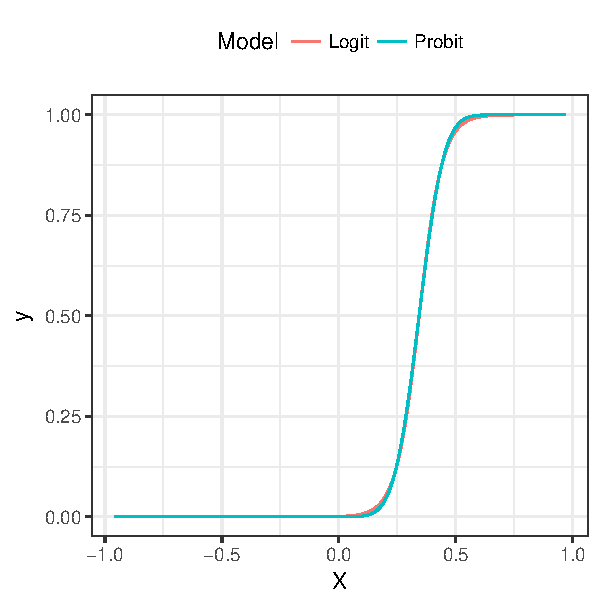
\includegraphics[width=\linewidth]{Probit-Logit-Fitted.pdf}
	\caption{Comparison of Probit and Logit Curves}
	\label{fig:Probit-Logit-Fit}
\end{figure}

Each of the estimation models was able to successfully select its own data generation process the majority of the time. The average model selection probability of the probit model under the probit data generation process was 0.679, and the probit marginal likelihood exceeded the logit marginal likelihood 96\% of the time in that case. Conversely, the average model selection probability of the logit model under the logit data generation process was 0.541, and the logit was more likely than the probit in 67\% of the simulations. While this result may initially seem underwhelming, it is made more impressive the remarkable similarity in probit and logit curves, as shown in \Cref{fig:Probit-Logit-Fit}. Further, as mentioned in the previous subsection, model comparison between logit and probit models has presented a struggle for both classical and Bayesian methods. As shown in this example, iterative KDE opens the possibility of comparing these models in a statistically meaningful way.

\section{Conclusion}

\bibliographystyle{chicago}
\bibliography{Iterative_ML}

\end{document}
